
\section{Análisis de herramientas y tecnologías}
A continuacón se presenta un análisis, comparación y selecccion de las 
herramientas y tecnologías a  utilizar en el desarrollo de este proyecto 
,así como las razones que justifican su elección considerando aspectos 
técnicos, económicos y de disponibilidad en base a las necesidades del 
proyecto. Se incluyen herramientas de hardware, software y plataformas 
evalúando las ventajas y desventajas
de cada una, así como su adecuación al proyecto.
\section{Análisis del Módulo 1}
En esta sección se presenta un análisis,comparacción y selección tanto de los sensores,como del microcontrolador 
a implementar en el Módulo 1 de este proyecto mediante una tabla comparativa de las diferentes opciones
disponibles en el mercado que cumplen con los requerimientos funcionales del proyecto.
A continuació se describen los componentes principales del Módulo 1:
\subsection{Sensor de pH}
Para medir el pH del kéfir de leche durante la fermentación, se
utilizará un sensor de pH analógico. Este sensor debe ser capaz de proporcionar
una salida de voltaje proporcional al valor de pH medido.
Para la selección del sensor de pH, se consideraron los siguientes
criterios en base a los requeriminetos funcionales del
proyecto:
\begin{itemize}
    \item \textbf{No contaminante:} El sensor debe ser adecuado para su uso en
    líquidos, en especial, en fermentaciones y no debe estar hecho de un material que pueda
    contaminar el kéfir por lo que es recomendado que este hecho de algun polimero de grado alimenticio, vidiro o de ceramica.
    \item \textbf{Rango de medición:}El sensor debe cubrir el rango de pH esperado durante
    la fermentación del kéfir de leche, que típicamente varía entre 6.8(inicial) y
    4.6(final).
    \item \textbf{Precisión:}El sensor debe tener una precisión adecuada para detectar
    cambios pequeños en el pH, idealmente con una precisión de ±0.1 pH.
    \item \textbf{Salida:}Se consideraron sensores con conectores estándar (como BNC)
    para facilitar una salida digital y una conexión con el microcontrolador.
    \item \textbf{Temperatura de operación:}El sensor debe ser capaz de operar en el
    rango de temperatura esperado durante la fermentación (18-30 °C).
    \item \textbf{Disponibilidad y costo:}Se consideraron sensores que sean fácilmente
    adquiribles y con un costo razonable para el proyecto.
\end{itemize}
A continuación se presentan la  con diferentes sensores de pH
considerados para el proyecto:


\begin{landscape}
\begin{table}[h!]
    \centering
    \small
% Anchos de columna reducidos para encoger la tabla horizontalmente.
\begin{tabular}{|P{2.2cm}|P{1.2cm}|P{1.2cm}|P{2.2cm}|P{1.0cm}|P{1.2cm}|P{1.8cm}|P{1.5cm}|P{1.5cm}|P{1.4cm}|P{1.4cm}|P{2.0cm}|}
\hline
% FILA DE ENCABEZADOS
\textbf{Modelo} & 
\textbf{Rangos de medición pH} & 
\textbf{Voltaje} & 
\textbf{Referencia} & 
\textbf{Pre- cisión} & 
\textbf{Tiempo de Respuesta} & 
\textbf{Temp. de operación C} & 
\textbf{Cuerpo} & 
\textbf{Punta} & 
\textbf{Tipo de Salida} & 
\textbf{Precio (MXN)} & 
\textbf{Imagen} \\ 
\hline
% DATOS - Heredan el tamaño \small
Hanna Instruments-FC200B\cite{zotero-item-24} & 0 a 12 & 3.3V-5.5V & Ag/AgC (Plata/cloruro de plata) & 0,1 & N/A & 0 a 50 & PVDF & Cónica de vidrio & BNC & \$5233.92 &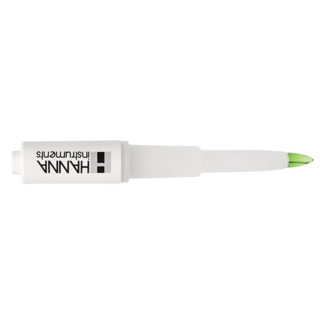
\includegraphics[width=20mm]{./Imagenes/Módulo1/pH/S1.jpg} \\ \hline

Milwaukee SE-220\cite{zotero-item-27} & 0 a 14 & 3.3V-5.5V & doble unión Ag/AgC & 0,02 & N/A & -5 a 70 & Resina-PEI & esférica & BNC & \$1762 & 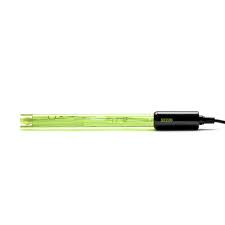
\includegraphics[width=20mm]{./Imagenes/Módulo1/pH/images.jpeg} \\ \hline

Atlas Científic-ENV-40-pH \cite{zotero-item-35} & 0 a 14 & 3.3V-5.5V & doble unión Ag/AgC & 0,001 & 1 seg. & 5 - 99 & Polica- rbonato & esférica & BNC & \$3000-4000 & 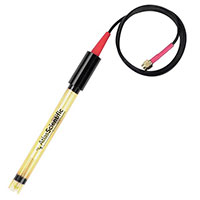
\includegraphics[width=20mm]{./Imagenes/Módulo1/pH/MFG_ENV-40-pH_primary_sml.jpg} \\ \hline

Atlas Científic-ENV-30-pH \cite{zotero-item-33} & 2 a 12 & 3.3V-5.5V & Ag/AgC & 0.1 & 4 seg. & 1-60 & Polica- rbonato & esférica & BNC & \$1000-2000 & 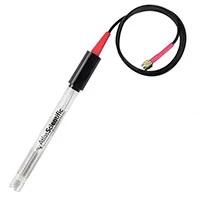
\includegraphics[width=20mm]{./Imagenes/Módulo1/pH/MFG_ENV-30-pH _primary_sml.jpg} \\ \hline

PH-E201C \cite{zotero-item-47} & 0 a 14 & 5V & Ag/AgCl & 0.02 & 5 seg. & 0-80 & Polica- rbonato & esférica & BNC & \$250-500 & 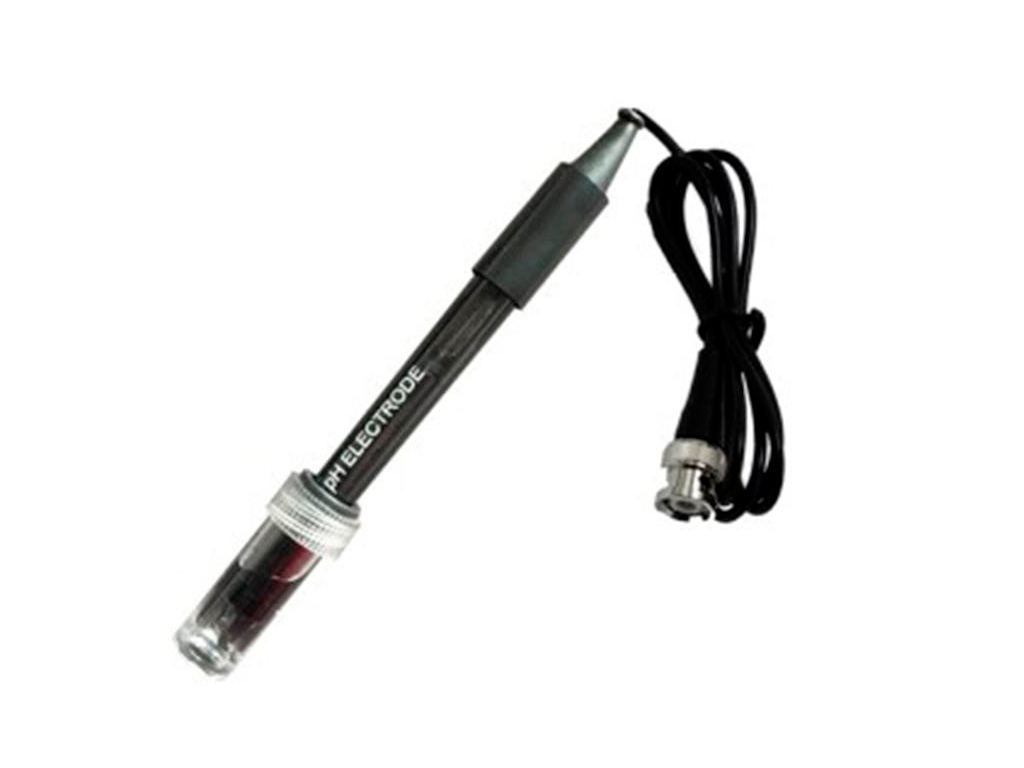
\includegraphics[width=20mm]{./Imagenes/Módulo1/pH/electrodo-para-medición-de-ph-e201c.jpg} \\ \hline
\end{tabular}
\caption{Sensores de pH.}
\label{tab:sensorespH}
\end{table}
\end{landscape}

Tras un análisis comparativo detallado de los sensores presentados en la Tabla \ref{tab:sensorespH}, se ha determinado que el electrodo PH-E201C \cite{zotero-item-47} es la opción más viable para la integración en este proyecto. Si bien los modelos alternativos cumplen con la mayoría de los requerimientos funcionales, el PH-E201C ofrece una combinación óptima de rendimiento y coste. Este sensor destaca por su excelente precisión de 0.02 unidades de pH y un tiempo de respuesta rápido de 5 segundos. Además de estas características técnicas sólidas, su bajo coste y alta disponibilidad en el mercado lo convierten en la solución más accesible y eficiente frente a las opciones de mayor precio.

\subsection{Sensor de Temperatura}
Para medir la temperatura del kéfir de leche durante la fermentación, se
utilizará un sensor de temperatura digital. Este sensor debe ser capaz de
proporcionar una lectura precisa de la temperatura en grados Celsius.
Para la selección del sensor de temperatura, se consideraron los siguientes
criterios en base a los requeriminetos funcionales del
proyecto:
\begin{itemize}
    \item \textbf{No contaminante:} El sensor debe ser adecuado para su uso en
    líquidos, en especial, en fermentaciones y no debe estar hecho de un material que pueda
    contaminar el kéfir por lo que es recomendado que este hecho de acero inoxidable de grado alimenticio.
    \item \textbf{Rango de medición:}El sensor debe cubrir el rango de temperatura
    esperado durante la fermentación del kéfir de leche, que típicamente varía entre
    18 y 30 °C.
    \item \textbf{Precisión:}El sensor debe tener una precisión adecuada para detectar
    cambios pequeños en la temperatura, idealmente con una precisión de ±0.5 °C.
    \item \textbf{Salida:}Se consideraron sensores con salida digital (como I2C o
    1-Wire) para facilitar la integración con el microcontrolador.
    \item \textbf{Disponibilidad y costo:}Se consideraron sensores que sean fácilmente
    adquiribles y con un costo razonable para el proyecto.
\end{itemize}
A continuación se presentan la tabla diferentes sensores de temperatura
considerados para el proyecto:

\begin{table}[h!]
    \centering
    \resizebox{\textwidth}{!}{
\begin{tabular}{|m{2.5cm}|m{2.5cm}|m{1.8cm}|m{2.5cm}|m{3.5cm}|m{2cm}|m{2cm}|m{2cm}|}
\hline
\textbf{Modelo}  & \textbf{Rangos de medición} & \textbf{Voltaje} & \textbf{Material} & \textbf{Error} & \textbf{Tipo de salida} & \textbf{Precio (MXN)} & \textbf{Imagen} \\ \hline
DS18B20\cite{zotero-item-43} & –55 °C a 125 °C & 3.3–5.5 V & Acero inoxidable & \begin{tabular}[c]{@{}c@{}}–10 °C a 85 °C\\ ±0.5 °C\end{tabular} & 1-Wire & \$50–150 & 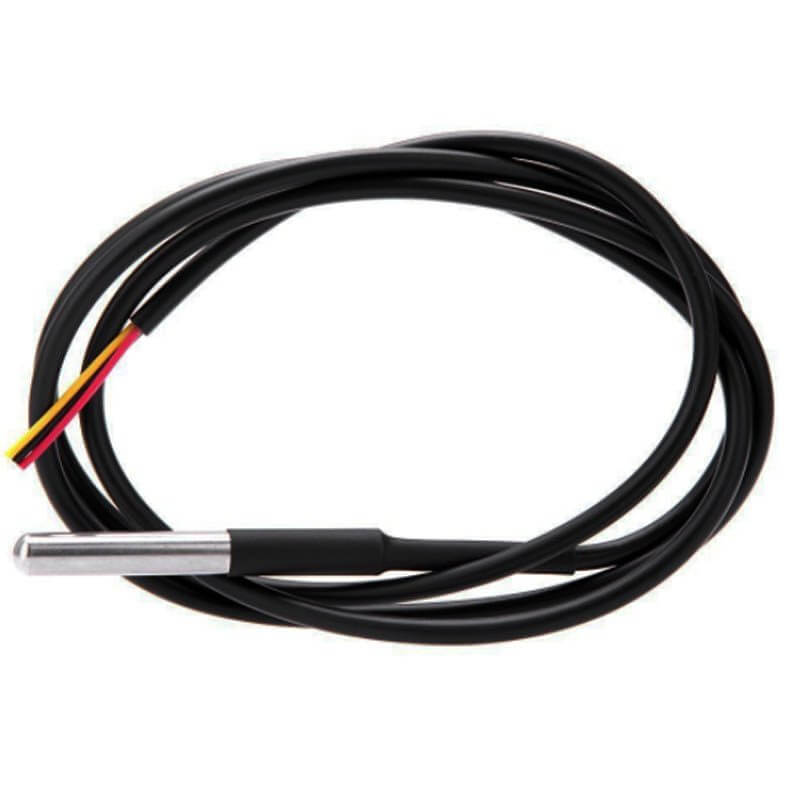
\includegraphics[width=20mm]{./Imagenes/Módulo1/Temperatura/t1.jpg} \\ \hline
E52-CA6DN 4M\cite{zotero-item-45} & 0–350 °C & 3.3–5.5 V & Acero inoxidable & \begin{tabular}[c]{@{}c@{}}0–333 °C\\ ±2.5 °C\end{tabular} & 1-Wire & \$2104 & 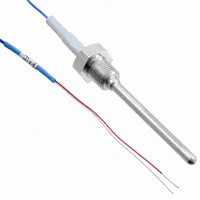
\includegraphics[width=20mm]{./Imagenes/Módulo1/Temperatura/t2.jpg} \\ \hline
\end{tabular}
    }
\caption{Tabla comparativa de sensores de temperatura.}
\label{tab:sensoresTemp}
\end{table}

En base a los sensores presentados en la Tabla \ref{tab:sensoresTemp}, 
el sensor DS18B20 \cite{zotero-item-43} se integra mucho mejor al proyecto a diferencia de los otros sensores,
ya que presenta un índice de error de solo +/-0.5C combinada con su bajo coste lo convierte en la elección más eficiente.

\subsection{Sensor de $CO_{2}$}
Para medir la concentración de dióxido de carbono ($CO_{2}$) en el ambiente
circundante al kéfir de leche durante la fermentación, se utilizará un
sensor de $CO_{2}$. Este sensor debe ser capaz de proporcionar una lectura precisa
de la concentración de $CO_{2}$ en partes por millón (ppm).
Para la selección del sensor de $CO_{2}$, se consideraron los siguientes
criterios en base a los requeriminetos funcionales del
proyecto:
\begin{itemize}
    \item \textbf{Rango de medición:}El sensor debe cubrir el rango de concentración
    de $CO_{2}$ esperado durante la fermentación del kéfir de leche, que típicamente varía
    entre 0 y 5000 ppm.
    \item \textbf{Precisión:}El sensor debe tener una precisión adecuada para detectar
    cambios pequeños en la concentración de $CO_{2}$, idealmente con una precisión de ±50 ppm.
    \item \textbf{Salida:}Se consideraron sensores con salida digital (como I2C o
    UART) para facilitar la integración con el microcontrolador.
    \item \textbf{Temperatura de operación:}El sensor debe ser capaz de operar en el
    rango de temperatura esperado durante la fermentación (18-30 °C).
    \item \textbf{Disponibilidad y costo:}Se consideraron sensores que sean fácilmente
    adquiribles y con un costo razonable para el proyecto.
\end{itemize}
A continuación se presentan la tabla diferentes sensores de $CO_{2}$
considerados para el proyecto:


\begin{table}[h!]
    \centering
    \small % Tamaño de fuente pequeño para que quepa
 \resizebox{\textwidth}{!}{
% Definición de 7 columnas (m{ancho}) para el texto/datos + 1 columna de imagen = 8 COLUMNAS TOTALES
\begin{tabular}{|m{2.5cm}|m{2.5cm}|m{1.8cm}|m{2.5cm}|m{3.5cm}|m{2cm}|m{2cm}|} 
\hline
% LÍNEA DEL ENCABEZADO CORREGIDA (sin espacios innecesarios dentro de \$)
\textbf{Sensor} & \textbf{Precisión} & \textbf{Rango de medición} & \textbf{Temp. de operación °C} & 
\textbf{Voltaje / Consumo} & \textbf{Precio aprox. (MXN)} & \textbf{Imagen} \\ 
\hline
% Filas de datos (revisadas)
MQ-135\cite{zotero-item-48} & N/A & 10-1000 ppm (estimado, otros gases) & -20 a +50°C & 5 V & \$100-200 & 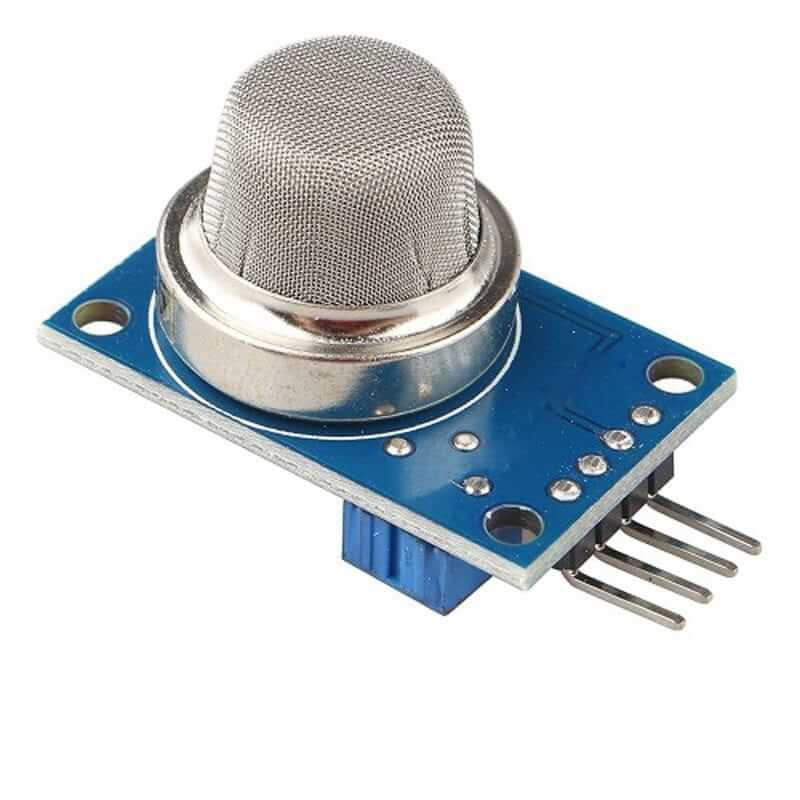
\includegraphics[width=20mm]{./Imagenes/Módulo1/Gas/mq135.jpg}\\ \hline

MH-Z19 / MH-Z19B\cite{zotero-item-50}& +/-(50ppm+5\%) & 400-10000 ppm & -10 a 50°C & 3.6-5.5 V & \$700-1700 & 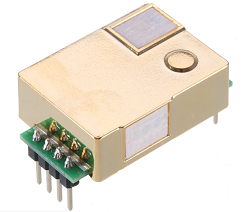
\includegraphics[width=20mm]{./Imagenes/Módulo1/Gas/HX-Z19.jpg} \\ \hline

SCD30 (Sensirion)\cite{zotero-item-52} &+/- (30ppm+3\%)  & 0-40000 ppm & 0 a 50°C & 3.3-5.5 V & \$780-1500 & 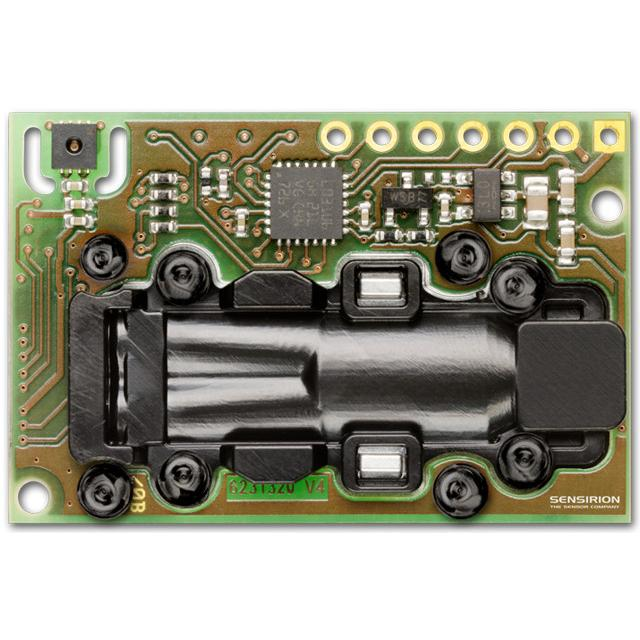
\includegraphics[width=20mm]{./Imagenes/Módulo1/Gas/scd30-5.jpg} \\ \hline

MG-811\cite{zotero-item-54} & +/- (30ppm+5\%)  & 350-10000 ppm & 20 a 50°C & 5-6 V& \$600-740 & 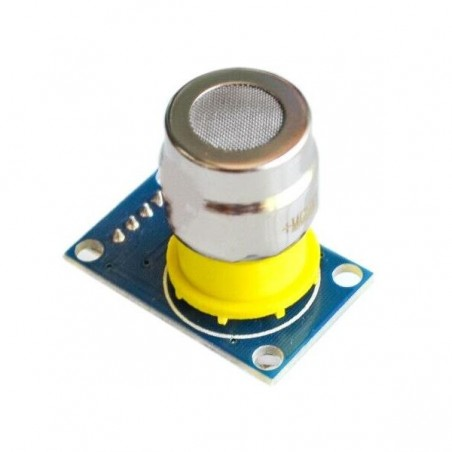
\includegraphics[width=20mm]{./Imagenes/Módulo1/Gas/md-mg81.jpg} \\ \hline
\end{tabular}
    }
    \caption{Sensores de $CO_{2}$}
    \label{tab:sensoresCO2}
\end{table}
Uno de los par\'ametros m\'as dif\'iciles de medir en la fermentaci\'on es 
el \textbf{${CO}_{2}$}. Dado que la fermentaci\'on del k\'efir libera grandes 
cantidades de este gas, se requiere un sensor con una excelente precisi\'on y un 
amplio rango de medici\'on. En base a los sensores presentados en la Tabla \ref{tab:sensoresCO2},
el sensor \textbf{SCD30 (Sensirion)} \cite{zotero-item-52} es la mejor opci\'on para el proyecto.
Esto se debe a que presenta un \'indice de error de solo +/-(30ppm+3\%) y un rango de 
medici\'on superior (0-40,000 ppm). Aunque no es el m\'as barato, su especializaci\'on en 
la medici\'on de ${CO}_{2}$ evita los problemas de precisi\'on que tendr\'ian otros sensores 
de menor calidad, como el MQ-135 (sensible a otros gases), o el rango limitado de los modelos MG-811 
y MH-Z19 en el contexto espec\'ifico de la fermentaci\'on del k\'efir.



\subsection{Microcontrolador}
En base a los sensores seleccionados y los requerimientos del proyecto, seconsideraron los siguientes microcontroladores:
\begin{table}[h]
    \centering
    \caption{Resumen de Frameworks de Backend de Python para IoT}
    \label{tab:backend_resumen_corregido}
    \begin{tabular}{|l|l|l|l|}
        \hline
        \textbf{Característica} & \textbf{FastAPI} & \textbf{Flask} & \textbf{Django} \\
        \hline
        \textbf{Tipo de Framework} & Asíncrono (API-first) & Microframework & Full-Stack \\
        \hline
        \textbf{Rendimiento} & Excelente & Bueno & Aceptable \\
        \hline
        \textbf{Lógica Asíncrona} & Nativa & Requiere Ext. & Requiere Config. \\
        \hline
        \textbf{Gestión de Usuarios} & Manual/Ext. & Requiere Ext. & Integrada \\
        \hline
        \textbf{Documentación API} & Automática & Requiere Ext. & Requiere Ext. \\
        \hline
        \textbf{Curva de Aprendizaje} & Media & Baja & Alta \\
        \hline
    \end{tabular}
\end{table}

\subsection{Formato de envio de datos}
Para el envío de datos desde los sensores al microcontrolador, se
consideraron los siguientes formatos de comunicación:
\begin{table}[h]
\centering
\caption{Formatos de Datos Comunes (Resumen)}
\label{tab:data_formats}
\begin{tabular}{|l|l|l|l|}
\hline
\textbf{Formato} & \textbf{Tipo} & \textbf{Ventaja Clave} & \textbf{Desventaja Clave} \\
\hline
\textbf{JSON} & Texto (Clave-Valor) & Fácil de usar, estándar de la industria. & Más verboso que binario (mayor tamaño). \\
\hline
\textbf{XML} & Texto (Etiquetas) & Estructura jerárquica y flexible. & Más verboso que JSON (mayor tamaño). \\
\hline
\textbf{Protobuf} & Binario & Muy compacto y eficiente en velocidad. & No es legible por humanos (requiere compilación). \\
\hline
\textbf{CSV} & Texto (Delimitado) & Extremadamente simple de implementar. & Carece de estructura para datos complejos. \\
\hline
\textbf{Binario} & Binario (Custom) & Máxima eficiencia en tamaño (cero sobrecarga). & Requiere implementación personalizada compleja. \\
\hline
\end{tabular}
\end{table}

\subsection{Protocolo de Comunicación}
Para la comunicación entre el microcontrolador y la base de datos se consideraron los siguientes protocolos de comunicación:
\begin{table}[h]
\centering
\caption{Comparación de Protocolos de Comunicación para ESP32}
\label{tab:protocol_comparison}
\begin{tabular}{|l|l|l|l|}
\hline
\textbf{Protocolo} & \textbf{Arquitectura} & \textbf{Eficiencia/Uso} & \textbf{Mejor para} \\
\hline
\textbf{MQTT} & Publicador/Suscriptor & Muy eficiente, baja latencia/ancho de banda. & Monitoreo con muchos sensores (\textbf{IoT}). \\
\hline
\textbf{HTTP/HTTPS} & Solicitud/Respuesta & Menos eficiente (cabeceras grandes). & Interacciones \textbf{Web}, peticiones únicas (API). \\
\hline
\textbf{CoAP} & Solicitud/Respuesta (Ligero) & Muy eficiente, diseñado para redes con restricciones. & \textbf{Dispositivos muy limitados} o redes \textbf{LPWAN}. \\
\hline
\textbf{WebSocket} & Cliente/Servidor (Persistente) & Bajo overhead, conexión \textbf{bidireccional} continua. & Actualizaciones en tiempo real (\textbf{Dashboards}). \\
\hline
\textbf{TCP/UDP} & Punto a Punto (Raw) & Máximo control (TCP seguro, UDP rápido/sin garantía). & Transmisión de datos \textbf{personalizada} o streaming. \\
\hline
\end{tabular}
\end{table}
\subsection{Fuente de alimentación}

\section{Análisis del Módulo 2}
Para llevar acabo el analisis de datos en base a los requerimientos funcionales se 
consideran los siguientes lenguajes:
\begin{table}[h]
    \centering
    \caption{Comparativa de Lenguajes para Lógica Difusa y JSON}
    \label{tab:lenguajes_fuzzy}
    \begin{tabular}{|l|c|c|c|l|}
        \hline
        \textbf{Lenguaje} & \textbf{Adecuación para Lógica Difusa} & \textbf{Librería Principal} & \textbf{Manejo de JSON} & \textbf{Uso Típico en el Proyecto} \\
        \hline
        \textbf{Python} & Excelente & \texttt{scikit-fuzzy} & Excelente (Nativo) & Backend de Análisis, API, y lógica difusa \\
        \hline
        \textbf{R} & Adecuada/Buena & \texttt{sets}, \texttt{FuzzyR} & Buena (Con \texttt{jsonlite}) & Análisis Estadístico Avanzado \\
        \hline
        \textbf{C\#} & Adecuada & \texttt{FuzzyLogic}, \texttt{FuzzySharp} & Muy Buena (Nativo con \texttt{System.Text.Json}) & Aplicaciones de Escritorio/Servidor (.NET) \\
        \hline
    \end{tabular}
\end{table}
\section{Análisis del Módulo 3}
Para llevar acabo el analisis de datos en base a los requerimientos funcionales se 
consideran los siguientes lenguajes:
\begin{table}[h]
    \centering
    \caption{Resumen de Bases de Datos para Proyectos IoT}
    \label{tab:bd_resumen}
    \begin{tabular}{|l|l|l|l|}
        \hline
        \textbf{Característica} & \textbf{InfluxDB (Series de Tiempo)} & \textbf{PostgreSQL (Relacional)} & \textbf{MongoDB (Documentos)} \\
        \hline
        \textbf{Uso Principal en IoT} & Datos de Sensores (pH, Temp, etc.) & Gestión de Usuarios y Metadatos & Datos Semiestructurados \\
        \hline
        \textbf{Optimización TS*} & \textbf{Excelente} (Diseño Nativo) & Baja (Requiere Extensiones) & Baja (No Optimizado) \\
        \hline
        \textbf{Manejo de JSON} & Muy Buena (API y Formato) & \textbf{Excelente} (\texttt{jsonb} Nativo) & \textbf{Excelente} (Formato Nativo) \\
        \hline
        \textbf{Flexibilidad Esquema} & Baja (Esquema Fijo) & Baja (Esquema Estricto) & \textbf{Excelente} (Esquema Dinámico) \\
        \hline
        \textbf{Escalabilidad} & Alta & Media-Alta & \textbf{Alta} \\
        \hline
        \multicolumn{4}{l}{\small *TS: Series de Tiempo} \\
    \end{tabular}
\end{table}
\section{Análisis del Módulo 4}
En esta sección se presenta un análisis comparativo de las opciones de frontend para el monitoreo del sistema IoT, considerando las necesidades específicas del proyecto, como la visualización de datos en tiempo real, la personalización de la interfaz y la integración con la base de datos InfluxDB.
Se evaluaron dos opciones principales: Grafana y un framework de desarrollo web como React o Vue
\begin{table}[h]
    \centering
    \caption{Resumen de Opciones de Frontend para Monitoreo IoT}
    \label{tab:frontend_resumen}
    \begin{tabular}{|l|l|l|l|}
        \hline
        \textbf{Característica} & \textbf{Grafana}  & \textbf{React (o Vue.js)}  & \textbf{Apto para tu Proyecto} \\
        \hline
        \textbf{Tipo de Solución} & Herramienta de Visualización & Framework de Desarrollo & \\
        \hline
        \textbf{Personalización de UI} & Limitada (Paneles y Plugins) & \textbf{Total} & \multicolumn{1}{l|}{} \\
        \hline
        \textbf{Integración con InfluxDB} & \textbf{Nativa y Directa} & Vía \textbf{Backend API} & \multicolumn{1}{l|}{} \\
        \hline
        \textbf{Gestión de Usuarios Específica} & Requiere Plugins/Configuración Compleja & \textbf{Ideal} (Manejada por Backend) & \multicolumn{1}{l|}{} \\
        \hline
        \textbf{Velocidad de Desarrollo} & \textbf{Rápida} (Dashboard Básico) & Lenta (Aplicación Completa) & \multicolumn{1}{l|}{} \\
        \hline
        \textbf{Recomendación} & Pruebas y Visualización Básica & \textbf{Desarrollo de Aplicación Completa} & \textbf{React (o Vue.js)} \\
        \hline
    \end{tabular}
\end{table}
\section{Framework}
En esta sección se presenta un análisis comparativo de los principales frameworks de backend en Python, evaluando su idoneidad para el desarrollo de una API RESTful que maneje la lógica del sistema IoT, la comunicación con la base de datos InfluxDB y la gestión de usuarios.
\begin{table}[h]
    \centering
    \caption{Resumen de Frameworks de Backend de Python para IoT}
    \label{tab:backend_resumen}
    \begin{tabular}{|l|l|l|l|}
        \hline
        \textbf{Característica} & \textbf{FastAPI}  & \textbf{Flask}  & \textbf{Django} \\
        \hline
        \textbf{Tipo de Framework} & Asíncrono (API-first) & Microframework & Full-Stack \\
        \hline
        \textbf{Rendimiento} & \textbf{Excelente} (El más rápido) & Bueno & Aceptable \\
        \hline
        \textbf{Lógica Asíncrona} & \textbf{Nativa} (Ideal para MQTT) & Requiere Ext. & Requiere Config. \\
        \hline
        \textbf{Gestión de Usuarios} & Requiere Desarrollo Manual & Requiere Ext. & \textbf{Integrada} \\
        \hline
        \textbf{Documentación API} & \textbf{Automática (Swagger/OpenAPI)} & Requiere Ext. & Requiere Ext. \\
        \hline
        \textbf{Curva de Aprendizaje} & Media & \textbf{Baja} & Alta \\
        \hline
        \textbf{Recomendación para IoT} & \textbf{Mejor Opción} (Rendimiento y API) & Buena Opción (Simplicidad) & No Recomendado (Sobrecarga) \\
        \hline
    \end{tabular}
\end{table}
\section{Servidor}
